\documentclass[]{article}
\usepackage{lmodern}
\usepackage{amssymb,amsmath}
\usepackage{ifxetex,ifluatex}
\usepackage{fixltx2e} % provides \textsubscript
\ifnum 0\ifxetex 1\fi\ifluatex 1\fi=0 % if pdftex
  \usepackage[T1]{fontenc}
  \usepackage[utf8]{inputenc}
\else % if luatex or xelatex
  \ifxetex
    \usepackage{mathspec}
  \else
    \usepackage{fontspec}
  \fi
  \defaultfontfeatures{Ligatures=TeX,Scale=MatchLowercase}
\fi
% use upquote if available, for straight quotes in verbatim environments
\IfFileExists{upquote.sty}{\usepackage{upquote}}{}
% use microtype if available
\IfFileExists{microtype.sty}{%
\usepackage{microtype}
\UseMicrotypeSet[protrusion]{basicmath} % disable protrusion for tt fonts
}{}
\usepackage[margin=1in]{geometry}
\usepackage{hyperref}
\hypersetup{unicode=true,
            pdftitle={Linear Regression: MPG in the Motor Trend Cars Dataset},
            pdfauthor={Paul Clark},
            pdfborder={0 0 0},
            breaklinks=true}
\urlstyle{same}  % don't use monospace font for urls
\usepackage{color}
\usepackage{fancyvrb}
\newcommand{\VerbBar}{|}
\newcommand{\VERB}{\Verb[commandchars=\\\{\}]}
\DefineVerbatimEnvironment{Highlighting}{Verbatim}{commandchars=\\\{\}}
% Add ',fontsize=\small' for more characters per line
\usepackage{framed}
\definecolor{shadecolor}{RGB}{248,248,248}
\newenvironment{Shaded}{\begin{snugshade}}{\end{snugshade}}
\newcommand{\KeywordTok}[1]{\textcolor[rgb]{0.13,0.29,0.53}{\textbf{{#1}}}}
\newcommand{\DataTypeTok}[1]{\textcolor[rgb]{0.13,0.29,0.53}{{#1}}}
\newcommand{\DecValTok}[1]{\textcolor[rgb]{0.00,0.00,0.81}{{#1}}}
\newcommand{\BaseNTok}[1]{\textcolor[rgb]{0.00,0.00,0.81}{{#1}}}
\newcommand{\FloatTok}[1]{\textcolor[rgb]{0.00,0.00,0.81}{{#1}}}
\newcommand{\ConstantTok}[1]{\textcolor[rgb]{0.00,0.00,0.00}{{#1}}}
\newcommand{\CharTok}[1]{\textcolor[rgb]{0.31,0.60,0.02}{{#1}}}
\newcommand{\SpecialCharTok}[1]{\textcolor[rgb]{0.00,0.00,0.00}{{#1}}}
\newcommand{\StringTok}[1]{\textcolor[rgb]{0.31,0.60,0.02}{{#1}}}
\newcommand{\VerbatimStringTok}[1]{\textcolor[rgb]{0.31,0.60,0.02}{{#1}}}
\newcommand{\SpecialStringTok}[1]{\textcolor[rgb]{0.31,0.60,0.02}{{#1}}}
\newcommand{\ImportTok}[1]{{#1}}
\newcommand{\CommentTok}[1]{\textcolor[rgb]{0.56,0.35,0.01}{\textit{{#1}}}}
\newcommand{\DocumentationTok}[1]{\textcolor[rgb]{0.56,0.35,0.01}{\textbf{\textit{{#1}}}}}
\newcommand{\AnnotationTok}[1]{\textcolor[rgb]{0.56,0.35,0.01}{\textbf{\textit{{#1}}}}}
\newcommand{\CommentVarTok}[1]{\textcolor[rgb]{0.56,0.35,0.01}{\textbf{\textit{{#1}}}}}
\newcommand{\OtherTok}[1]{\textcolor[rgb]{0.56,0.35,0.01}{{#1}}}
\newcommand{\FunctionTok}[1]{\textcolor[rgb]{0.00,0.00,0.00}{{#1}}}
\newcommand{\VariableTok}[1]{\textcolor[rgb]{0.00,0.00,0.00}{{#1}}}
\newcommand{\ControlFlowTok}[1]{\textcolor[rgb]{0.13,0.29,0.53}{\textbf{{#1}}}}
\newcommand{\OperatorTok}[1]{\textcolor[rgb]{0.81,0.36,0.00}{\textbf{{#1}}}}
\newcommand{\BuiltInTok}[1]{{#1}}
\newcommand{\ExtensionTok}[1]{{#1}}
\newcommand{\PreprocessorTok}[1]{\textcolor[rgb]{0.56,0.35,0.01}{\textit{{#1}}}}
\newcommand{\AttributeTok}[1]{\textcolor[rgb]{0.77,0.63,0.00}{{#1}}}
\newcommand{\RegionMarkerTok}[1]{{#1}}
\newcommand{\InformationTok}[1]{\textcolor[rgb]{0.56,0.35,0.01}{\textbf{\textit{{#1}}}}}
\newcommand{\WarningTok}[1]{\textcolor[rgb]{0.56,0.35,0.01}{\textbf{\textit{{#1}}}}}
\newcommand{\AlertTok}[1]{\textcolor[rgb]{0.94,0.16,0.16}{{#1}}}
\newcommand{\ErrorTok}[1]{\textcolor[rgb]{0.64,0.00,0.00}{\textbf{{#1}}}}
\newcommand{\NormalTok}[1]{{#1}}
\usepackage{longtable,booktabs}
\usepackage{graphicx,grffile}
\makeatletter
\def\maxwidth{\ifdim\Gin@nat@width>\linewidth\linewidth\else\Gin@nat@width\fi}
\def\maxheight{\ifdim\Gin@nat@height>\textheight\textheight\else\Gin@nat@height\fi}
\makeatother
% Scale images if necessary, so that they will not overflow the page
% margins by default, and it is still possible to overwrite the defaults
% using explicit options in \includegraphics[width, height, ...]{}
\setkeys{Gin}{width=\maxwidth,height=\maxheight,keepaspectratio}
\IfFileExists{parskip.sty}{%
\usepackage{parskip}
}{% else
\setlength{\parindent}{0pt}
\setlength{\parskip}{6pt plus 2pt minus 1pt}
}
\setlength{\emergencystretch}{3em}  % prevent overfull lines
\providecommand{\tightlist}{%
  \setlength{\itemsep}{0pt}\setlength{\parskip}{0pt}}
\setcounter{secnumdepth}{5}
% Redefines (sub)paragraphs to behave more like sections
\ifx\paragraph\undefined\else
\let\oldparagraph\paragraph
\renewcommand{\paragraph}[1]{\oldparagraph{#1}\mbox{}}
\fi
\ifx\subparagraph\undefined\else
\let\oldsubparagraph\subparagraph
\renewcommand{\subparagraph}[1]{\oldsubparagraph{#1}\mbox{}}
\fi

%%% Use protect on footnotes to avoid problems with footnotes in titles
\let\rmarkdownfootnote\footnote%
\def\footnote{\protect\rmarkdownfootnote}

%%% Change title format to be more compact
\usepackage{titling}

% Create subtitle command for use in maketitle
\newcommand{\subtitle}[1]{
  \posttitle{
    \begin{center}\large#1\end{center}
    }
}

\setlength{\droptitle}{-2em}
  \title{Linear Regression: MPG in the Motor Trend Cars Dataset}
  \pretitle{\vspace{\droptitle}\centering\huge}
  \posttitle{\par}
  \author{Paul Clark}
  \preauthor{\centering\large\emph}
  \postauthor{\par}
  \predate{\centering\large\emph}
  \postdate{\par}
  \date{March 5, 2017}


\usepackage{float}
\let\origfigure\figure
\let\endorigfigure\endfigure
\renewenvironment{figure}[1][2] {
    \expandafter\origfigure\expandafter[H]
} {
    \endorigfigure
}

\begin{document}
\maketitle

\section{Executive Summary}\label{executive-summary}

For its 1974 edition, US magazine \emph{Motor Trend} has asked two
questions to be addressed using data on fuel consumption and 10 aspects
of automobile design and performance for 32 '73-'74 model autos.\\
\textbf{Questions}:

\begin{enumerate}
\def\labelenumi{\arabic{enumi}.}
\tightlist
\item
  ``Is an automatic or manual transmission better for MPG?''
\item
  ``Quantify the MPG-difference between automatic and manual
  transmissions.''
\end{enumerate}

\textbf{Variables:}

\begin{verbatim}
 [1] "mpg  Miles/(US) gallon"          "cyl  Num cylinders"             
 [3] "disp Displacement (cu.in.)"      "hp   Gross horsepower"          
 [5] "drat Rear axle ratio"            "wt   Weight (1000 lbs)"         
 [7] "qsec 1/4 mile time"              "vs   Engine(0=V,1=In-line)"     
 [9] "am   Transmission(0=auto,1=man)" "gear Num forward gears"         
[11] "carb Num carburetors"           
\end{verbatim}

We apply two \textbf{Approaches} to answering the questions:

\begin{enumerate}
\def\labelenumi{(\Alph{enumi})}
\tightlist
\item
  \textbf{T-test:} Analysis of the difference in means of \texttt{mpg}
  for the two transmission types
\item
  \textbf{Regression:} Investigation of the impact of other variables in
  adjusting or replacing the transmission effect.
\end{enumerate}

We have 5 \textbf{Conclusions} based on these analyses:

\begin{enumerate}
\def\labelenumi{\arabic{enumi}.}
\tightlist
\item
  The two groups come from populations with statistically different
  means.
\item
  If the data is representative, mean MPG of \emph{manual} transmission
  cars is approximately \textbf{7.2 MPG} higher than \emph{automatic},
  with a one-sided confidence interval of 3.9 MPG to infinity.
\item
  The adjustments of the transmission-type effect that are most helpful
  in prediction of \texttt{mpg} are \texttt{hp} and \texttt{wt}, both
  negative, and \texttt{vs}, which adds a positive adjustment for
  in-line engines as compared to V-type.
\item
  The \emph{transmission} effect, with \emph{horsepower}, \emph{weight},
  and \textbf{engine-type} held fixed, is approximately \textbf{2.4
  MPG}, with manual again having higher \texttt{mpg} than automatic.
  These other engineered effects are the sources of more of the
  difference in \texttt{mpg} (\textbf{4.8 MPG} worth) than transmission
  type alone.
\item
  Due to low significance of the \texttt{am} coefficient (\textbf{Std.
  Error} of X), we also investigate other models not constrained to
  include \texttt{am}. The best of these, selected via cross-validation,
  was \(E[mpg] = 39.6 -0.49\cdot carb -1.29\cdot cyl -3.16\cdot wt\).
\end{enumerate}

\section{Exploratory Data Analysis}\label{exploratory-data-analysis}

Note that for our analyses to be meaningful, this sample of 32 cars must
be representative of a larger, defined population of vehicles.

\begin{verbatim}
 [1] "Mazda RX4"           "Mazda RX4 Wag"       "Datsun 710"         
 [4] "Hornet 4 Drive"      "Hornet Sportabout"   "Valiant"            
 [7] "Duster 360"          "Merc 240D"           "Merc 230"           
[10] "Merc 280"            "Merc 280C"           "Merc 450SE"         
[13] "Merc 450SL"          "Merc 450SLC"         "Cadillac Fleetwood" 
[16] "Lincoln Continental" "Chrysler Imperial"   "Fiat 128"           
[19] "Honda Civic"         "Toyota Corolla"      "Toyota Corona"      
[22] "Dodge Challenger"    "AMC Javelin"         "Camaro Z28"         
[25] "Pontiac Firebird"    "Fiat X1-9"           "Porsche 914-2"      
[28] "Lotus Europa"        "Ford Pantera L"      "Ferrari Dino"       
[31] "Maserati Bora"       "Volvo 142E"         
\end{verbatim}

Note that the sample contains multiple Mercedes (7) and Mazdas (2). It
may enhance prediction to consider a ``Mercedes'' and/or ``Mazda''
effect in our modeling. However, in \textbf{Assumption (b)} below, we
restrict consideration to differences in fundamental engineering
variables, implicitly assuming that such differences explain any brand
specific effects.

In \textbf{Figure 1}, we examine integer predictors to decide whether to
treat them as factors. We find value in treating \texttt{cyl} and
\texttt{carb} as continuous: they show clear trends vs.~other variables.
And from a pairs plot, \textbf{Figure 2}, we see many strong
correlations, so model selection should consider variance inflation.

\section{Approach (A): T-test}\label{approach-a-t-test}

\textbf{Figure 3} shows that in this data, \texttt{mpg} varies with
\texttt{am}. Mean mileage for manual is \textbf{7.2 mpg} higher than
automatic. We compute p-value and confidence interval for the test of
manual transmission \emph{greater}.

\begin{Shaded}
\begin{Highlighting}[]
\NormalTok{t_test <-}\StringTok{ }\KeywordTok{t.test}\NormalTok{(mpg~am,}\DataTypeTok{data=}\NormalTok{mtcars,}\DataTypeTok{alternative=}\StringTok{'less'}\NormalTok{) }\CommentTok{#'less': level 2 is t.test base}
\CommentTok{# note: code for processing and formatting of output suppressed}
\end{Highlighting}
\end{Shaded}

\begin{verbatim}
p-value = 0.07%     95% confidence interval = 3.91 to Inf
\end{verbatim}

\textbf{Inference} Given the p-value, and assuming rough normality, we
are highly confident manual transmissions are associated with higher
fuel economy in the populations from which these samples were drawn.
Based on our sample values, the probability is only 1 in 20 that the
interval above 3.9 MPG does not contain our true difference in means.

\section{Approach (B): Regression}\label{approach-b-regression}

Approach \textbf{(B)} is under-specified. Having identified \texttt{mpg}
and \texttt{am} as of interest, the ``correct'' choice of model still
depends on selection of the appropriate subset of 9 other variables.
This should be a function of variable/model significance, but also
\emph{Motor Trend's} interests. For significance testing, manual
checking of p-values is in-viable: at least \(2^{9} = 512\) models with
single predictors exist. Therefore, to fully specify and make the
approach manageable, we must make additional assumptions.

\textbf{Assumptions}\\
In answering questions 1 ad 2, we assume \emph{Motor Trend} values the
following, in rough priority order:

\begin{enumerate}
\def\labelenumi{(\alph{enumi})}
\tightlist
\item
  Model parsimony/simplicity
\item
  Models with granular, causal variables that may clarify engineering
  trade-offs
\item
  Predictiveness: good generalizability outside the training sample
\end{enumerate}

\subsection{Model Search}\label{model-search}

\subsubsection{Test citations}\label{test-citations}

This is a test citation: (Breiman and Spector 1992), (Rao, Fung, and
Rosales 2008).

\subsubsection{Model search discussion}\label{model-search-discussion}

\begin{enumerate}
\def\labelenumi{\arabic{enumi}.}
\tightlist
\item
  Trade-off: Choose exact predictors during the inference process using
  R-squared for fixed number of predictors (do not detect over-fitting
  in predictor choice, only in number of predictors), or choose exact
  predictors during cross-validation (detect over-fitting in predictor
  choice, but potentially overfit the selection criterion)
\item
  LOOCV vs.~K-fold CV vs.~some point in between: a quagmire. Consensus
  is that positive bias on CV error is higher for K-fold, but no true
  consensus on the way variance changes on the spectrum of LOOCV to
  K-fold with small K.
\item
  Potential for over-fitting the selection criteria, especially for
  small sample size, leads to negative bias, but usage of low K for
  K-fold CV can have positive bias.
\item
  Use information theoretic result, or use cross-validation. Information
  theoretic result may be sufficient when precise variables chosen as
  part of inference on each fold, and there are indications that info
  theoretic results may be better than CV in such circumstances.
\end{enumerate}

Due to \textbf{(a)}, we consider no interactions. From \textbf{(b)}, we
exclude \texttt{qsec}, a summary metric. Due to \textbf{(c)}, we rank
models using the \textbf{AIC} metric, which estimates model
predictiveness outside the training sample. For OLS regression, the
metric is
\(n\cdot Log(\frac{\sum_{i=1}^n(y_{i}- \hat{y}_{i})^2}{n}) + 2k\), where
\(k =\) \# of parameters including estimate of residual error, an
overfitting penalty. In fact, we use \textbf{AICc}, which corrects the
penalty to be greater for small \(n\) by adding a term
\(\frac{2k(k + 1)}{{n}-{k}-1}\) (note that this term varies based on
model structure; this version only holds for Gaussian models). We use
automated search to make evaluation of all \(2^9\) models feasible.
Models are ranked from smallest to largest AICc. Only non-zero
coefficients are shown, and only models with the variable of interest
(\texttt{am}) are evaluated.

\begin{Shaded}
\begin{Highlighting}[]
\NormalTok{if (!}\StringTok{"MuMIn"} \NormalTok\StringTok{ }\KeywordTok{row.names}\NormalTok{(}\KeywordTok{installed.packages}\NormalTok{())) \{}\KeywordTok{install.packages}\NormalTok{(}\StringTok{"MuMIn"}\NormalTok{)\}}
\KeywordTok{library}\NormalTok{(MuMIn)}
\CommentTok{# preprocessing variables: remove unwanted perf. measure `qsec`; treat `gear` as factor}
\NormalTok{mtcars$qsec <-}\StringTok{ }\OtherTok{NULL}\NormalTok{; mtcars$gear <-}\StringTok{ }\KeywordTok{as.factor}\NormalTok{(mtcars$gear)}
\NormalTok{globalmodel <-}\StringTok{ }\KeywordTok{lm}\NormalTok{(mpg ~}\StringTok{ }\NormalTok{., }\DataTypeTok{data =} \NormalTok{mtcars, }\DataTypeTok{na.action =} \NormalTok{na.fail)}

\NormalTok{n_models <-}\StringTok{ }\DecValTok{2}\NormalTok{^(}\KeywordTok{length}\NormalTok{(}\KeywordTok{model.frame}\NormalTok{(globalmodel)) -}\StringTok{ }\DecValTok{1}\NormalTok{)}

\NormalTok{best_am_models <-}\StringTok{ }\KeywordTok{dredge}\NormalTok{(globalmodel, }\DataTypeTok{subset =} \NormalTok{~}\StringTok{ }\NormalTok{am) }\CommentTok{# considers only models with `am`}
\NormalTok{best_am_models[}\DecValTok{1}\NormalTok{:}\DecValTok{10}\NormalTok{,]}
\end{Highlighting}
\end{Shaded}

\begin{longtable}[]{@{}lllllllllllll@{}}
\caption{Best Models for MPG that Contain Transmission
Type}\tabularnewline
\toprule
& (Int) & am & carb & cyl & hp & vs & wt & df & logLik & AICc & delta &
weight\tabularnewline
\midrule
\endfirsthead
\toprule
& (Int) & am & carb & cyl & hp & vs & wt & df & logLik & AICc & delta &
weight\tabularnewline
\midrule
\endhead
322 & 34.0 & 2.08 & & & -0.037 & & -2.9 & 5 & -73.1 & 158.4 & 0.0 &
0.31\tabularnewline
264 & 36.9 & 1.78 & -0.75 & -1.20 & & & -2.5 & 6 & -72.0 & 159.4 & 0.9 &
0.20\tabularnewline
450 & 31.1 & 2.42 & & & -0.030 & 1.8 & -2.6 & 6 & -72.0 & 159.4 & 1.0 &
0.19\tabularnewline
326 & 36.1 & 1.48 & & -0.75 & -0.025 & & -2.6 & 6 & -72.1 & 159.6 & 1.2
& 0.17\tabularnewline
262 & 39.4 & 0.18 & & -1.51 & & & -3.1 & 5 & -74.0 & 160.3 & 1.9 &
0.12\tabularnewline
\bottomrule
\end{longtable}

\subsection{Model Inference \& Interpretation of
Coefficients}\label{model-inference-interpretation-of-coefficients}

We investigate values of the \texttt{am} coefficient for the top models.
Note the first 3 all round to 2, suggesting this is a good rough
estimate of the adjusted transmission effect. Although our top model is
only one AICc point lower than the next best model (model averaging is
suggested via the weights, for differences less than 2), we focus
attention on it, in the spirit of Assumption \textbf{(A)}.

\begin{longtable}[]{@{}lrr@{}}
\caption{Coefficients of Best Model Including Transmission
Type}\tabularnewline
\toprule
& Estimate & Std. Error\tabularnewline
\midrule
\endfirsthead
\toprule
& Estimate & Std. Error\tabularnewline
\midrule
\endhead
(Intercept) & 31.079 & 3.393\tabularnewline
am & 2.417 & 1.379\tabularnewline
hp & -0.030 & 0.011\tabularnewline
vs & 1.786 & 1.327\tabularnewline
wt & -2.591 & 0.917\tabularnewline
\bottomrule
\end{longtable}

The \(R^2\) of this top model is 85\%: it explains a high degree of
sample variance with only 3 covariates. The above table contains no
p-values, as after a search of \(2^9\) models, these would be inflated:
since the procedure only selects `good' models for consideration, we
need to control the ``False Discovery Rate'', which is the fraction of
\textbf{all rejected} null hypotheses which are false (i.e.,
\((False~Positives)/(False~ Positives + True~ Positives)\)), not just
\(\alpha\), which is the fraction of \textbf{all truly 0} results that
are rejected (i.e.,
\((False~Positives)/(False~ Positives + True~ Negatives)\)). However,
standard errors are provided. Increased engine \textbf{HP} accounts for
a decrease of 3.0 MPG per hundred HP, increased \textbf{weight} accounts
for a decrease of 2.6 MPG per thousand lbs, and \textbf{engine-type}
accounts for a difference of 1.8 MPG, with inline engines having higher
MPG than V-type engines. Note that significance of the the \texttt{am}
coefficient, 2.4, is low. The \emph{Estimate} over the \emph{Std.
Error}, or t-stat, is only 1.8. Two is near the \(\alpha=5\%\)
threshold. Given this, we investigate models that do \textbf{not}
include \texttt{am}. Here are the top 10 overall:

\begin{Shaded}
\begin{Highlighting}[]
\CommentTok{# given a model, calculates mean-squared test error for leave-k-out cross validation}
\NormalTok{lkocv <-}\StringTok{ }\NormalTok{function(lm_model, folds, mpg)\{}
        \NormalTok{n_folds <-}\StringTok{ }\KeywordTok{length}\NormalTok{(folds)}
        \NormalTok{modframe <-}\StringTok{ }\KeywordTok{model.frame}\NormalTok{(lm_model)}
        \NormalTok{n <-}\StringTok{ }\KeywordTok{names}\NormalTok{(modframe)}
        \NormalTok{sse <-}\StringTok{ }\KeywordTok{numeric}\NormalTok{(n_folds)}
        \NormalTok{if (}\KeywordTok{length}\NormalTok{(n) >}\StringTok{ }\DecValTok{1}\NormalTok{)\{}
                \NormalTok{f <-}\StringTok{ }\KeywordTok{as.formula}\NormalTok{(}\KeywordTok{paste}\NormalTok{(}\StringTok{"mpg ~"}\NormalTok{, }\KeywordTok{paste}\NormalTok{(n[!n %in%}\StringTok{ "mpg"}\NormalTok{], }
                                      \DataTypeTok{collapse =} \StringTok{" + "}\NormalTok{)))}
                \NormalTok{for (i in }\DecValTok{1}\NormalTok{:n_folds) \{}
                        \CommentTok{# iterate over all the folds, i; for each i...}
                        \CommentTok{# create model based on dataset leaving out fold i}
                        \NormalTok{trnd_model <-}\StringTok{ }\KeywordTok{lm}\NormalTok{(}\DataTypeTok{formula =} \NormalTok{f, }\DataTypeTok{data =} 
                                        \NormalTok{modframe[ -folds[[i]], ])}
                        \CommentTok{# calculate and store sum of squared errors for each fold i}
                        \NormalTok{sse[i] <-}\StringTok{ }\KeywordTok{sum}\NormalTok{((modframe[folds[[i]], }\StringTok{"mpg"}\NormalTok{] -}
\StringTok{                                        }\KeywordTok{predict}\NormalTok{(trnd_model, }\DataTypeTok{newdata =} 
                                                \NormalTok{modframe[folds[[i]],]))^}\DecValTok{2}\NormalTok{)}
                \NormalTok{\}}
                \NormalTok{\} else \{ }
                \NormalTok{f <-}\StringTok{ }\KeywordTok{as.formula}\NormalTok{(}\StringTok{"mpg ~ 1"}\NormalTok{)}
                \NormalTok{for (i in }\DecValTok{1}\NormalTok{:n_folds) \{}
                        \CommentTok{# iterate over all the folds, i; for each i...}
                        \CommentTok{# create model based on dataset leaving out fold i}
                        \NormalTok{trnd_model <-}\StringTok{ }\KeywordTok{lm}\NormalTok{(}\DataTypeTok{formula =} \NormalTok{f, }\DataTypeTok{data =} 
                                        \KeywordTok{data.frame}\NormalTok{(}\DataTypeTok{mpg =} \NormalTok{mpg[ -folds[[i]] ]))}
                        \CommentTok{# calculate and store sum of squared errors for each fold i}
                        \NormalTok{sse[i] <-}\StringTok{ }\KeywordTok{sum}\NormalTok{((mpg[ folds[[i]] ] -}
\StringTok{                                        }\KeywordTok{predict}\NormalTok{(trnd_model, }\DataTypeTok{newdata =} 
                                                \KeywordTok{data.frame}\NormalTok{(}\DataTypeTok{mpg =} \NormalTok{mpg[ folds[[i]] ])))^}\DecValTok{2}\NormalTok{)}
                \NormalTok{\}}
        \NormalTok{\}}
        \CommentTok{# sum up the squared errors across all folds, divide by n, get MSE}
        \NormalTok{mse_nobs <-}\StringTok{ }\KeywordTok{sum}\NormalTok{(sse)/}\KeywordTok{nrow}\NormalTok{(modframe)}
        \NormalTok{mse_nobs}
\NormalTok{\}}


\CommentTok{# function does n_iter iterations of cross-validation per fold, averages the results,}
\CommentTok{# returning out-of-sample r-squared}
\NormalTok{lkocv_iter <-}\StringTok{ }\NormalTok{function(lm_model, }\DataTypeTok{k.=} \NormalTok{k, }\DataTypeTok{n_iter.=}\NormalTok{n_iter, }\DataTypeTok{rseed. =} \NormalTok{rseed,}
                       \DataTypeTok{n_models. =} \NormalTok{n_models)}
\NormalTok{\{}
        \KeywordTok{set.seed}\NormalTok{(rseed.)}
        \NormalTok{modframe <-}\StringTok{ }\KeywordTok{model.frame}\NormalTok{(lm_model)}
        \NormalTok{mpg <-}\StringTok{ }\NormalTok{modframe$mpg}
        \NormalTok{dev_mean <-}\StringTok{ }\NormalTok{mpg -}\StringTok{ }\KeywordTok{mean}\NormalTok{(mpg)}
        \NormalTok{mse_iter <-}\StringTok{ }\KeywordTok{numeric}\NormalTok{(n_iter.)}
        \NormalTok{n_sample <-}\StringTok{ }\KeywordTok{nobs}\NormalTok{(lm_model)}
        \NormalTok{if (k. >}\StringTok{ }\DecValTok{1}\NormalTok{) \{}
                \NormalTok{for (i in }\DecValTok{1}\NormalTok{:n_iter.) \{}
                        \NormalTok{folds <-}\StringTok{ }\KeywordTok{split}\NormalTok{(}\KeywordTok{sample}\NormalTok{(n_sample), }\KeywordTok{gl}\NormalTok{(}\KeywordTok{ceiling}\NormalTok{(n_sample/k.),}
                                                            \NormalTok{k., n_sample))}
                        \CommentTok{# returns mean-squared-error of all observations in iteration i}
                        \NormalTok{mse_iter[i] <-}\StringTok{ }\KeywordTok{lkocv}\NormalTok{(}\DataTypeTok{lm_model =} \NormalTok{lm_model, }\DataTypeTok{folds =} \NormalTok{folds, mpg)}
                \NormalTok{\}}
        
        \NormalTok{\} else \{}
                \CommentTok{# leave-one-out cross-validation (loocv)}
                \NormalTok{h <-}\StringTok{ }\KeywordTok{lm.influence}\NormalTok{(lm_model)$hat}
                \NormalTok{mse_iter <-}\StringTok{ }\NormalTok{(}\KeywordTok{residuals}\NormalTok{(lm_model)/(}\DecValTok{1} \NormalTok{-}\StringTok{ }\NormalTok{h))^}\DecValTok{2}
        \NormalTok{\}}
        \NormalTok{if (.GlobalEnv$n %%}\StringTok{ }\DecValTok{10} \NormalTok{==}\StringTok{ }\DecValTok{0}\NormalTok{) }\KeywordTok{cat}\NormalTok{(}\DataTypeTok{sep =} \StringTok{""}\NormalTok{, }\StringTok{"}\CharTok{\textbackslash{}n}\StringTok{"}\NormalTok{)}
        \KeywordTok{assign}\NormalTok{(}\StringTok{"n"}\NormalTok{, .GlobalEnv$n +}\StringTok{ }\DecValTok{1}\NormalTok{, .GlobalEnv)}
        \NormalTok{if (.GlobalEnv$n <=}\StringTok{ }\NormalTok{n_models.) \{}
                \KeywordTok{cat}\NormalTok{(}\DataTypeTok{sep =} \StringTok{""}\NormalTok{, }\StringTok{"["}\NormalTok{, .GlobalEnv$n,}\StringTok{"/"}\NormalTok{, n_models.,}\StringTok{"]"}\NormalTok{)}
        \NormalTok{\}}
        \CommentTok{# 1 - out-of-sample R-squared}
        \KeywordTok{mean}\NormalTok{(mse_iter)/}\KeywordTok{mean}\NormalTok{(dev_mean^}\DecValTok{2}\NormalTok{)}
\NormalTok{\}}
\end{Highlighting}
\end{Shaded}

\subsubsection{Model Investigation: Leave K-out Cross
Validation}\label{model-investigation-leave-k-out-cross-validation}

\paragraph{Eight-Fold Cross
Validation}\label{eight-fold-cross-validation}

\begin{Shaded}
\begin{Highlighting}[]
\KeywordTok{assign}\NormalTok{(}\DataTypeTok{x =} \StringTok{"n"}\NormalTok{, }\DataTypeTok{value =} \DecValTok{0}\NormalTok{, }\DataTypeTok{envir =} \NormalTok{.GlobalEnv) }\CommentTok{# for running as RStudio NB/console }
\NormalTok{n_iter <-}\StringTok{ }\DecValTok{25}
\NormalTok{rseed <-}\StringTok{ }\DecValTok{19720921}
\NormalTok{k <-}\StringTok{ }\DecValTok{4}
\NormalTok{model_sel_leave4_out_df <-}\StringTok{ }\KeywordTok{dredge}\NormalTok{(globalmodel, }\DataTypeTok{rank =} \NormalTok{lkocv_iter)}
\KeywordTok{prnt_model_sel_table}\NormalTok{(model_sel_leave4_out_df, }\DataTypeTok{metric_name =} \StringTok{"1-Rsq_l4ocv"}\NormalTok{, }
                  \DataTypeTok{caption =} \StringTok{"Best Overall Models for MPG (L4OCV)"}\NormalTok{)}
\end{Highlighting}
\end{Shaded}

\paragraph{Leave One Out Cross
Validation}\label{leave-one-out-cross-validation}

\begin{Shaded}
\begin{Highlighting}[]
\KeywordTok{assign}\NormalTok{(}\DataTypeTok{x =} \StringTok{"n"}\NormalTok{, }\DataTypeTok{value =} \DecValTok{0}\NormalTok{, }\DataTypeTok{envir =} \NormalTok{.GlobalEnv)}
\NormalTok{metric_name <-}\StringTok{ "1-Rsq_loocv"}
\NormalTok{caption <-}\StringTok{ "Best Overall Models for MPG (LOOCV)"}
\NormalTok{rseed <-}\StringTok{ }\DecValTok{19720921}
\NormalTok{k <-}\StringTok{ }\DecValTok{1}
\NormalTok{n_iter <-}\StringTok{ }\DecValTok{1}
\NormalTok{model_sel_leave1_out_df <-}\StringTok{ }\KeywordTok{dredge}\NormalTok{(globalmodel, }\DataTypeTok{rank =} \NormalTok{lkocv_iter)}
\end{Highlighting}
\end{Shaded}

\begin{Shaded}
\begin{Highlighting}[]
\KeywordTok{prnt_model_sel_table}\NormalTok{(model_sel_leave1_out_df, }\DataTypeTok{metric_name =} \StringTok{"1-Rsq_loocv"}\NormalTok{,}
                     \DataTypeTok{caption =} \NormalTok{caption)}
\end{Highlighting}
\end{Shaded}

\begin{longtable}[]{@{}llllllllllllll@{}}
\caption{Best Overall Models for MPG (LOOCV)}\tabularnewline
\toprule
& (Int) & am & carb & cyl & disp & drat & gear & hp & vs & wt & df &
1-Rsq\_loocv & delta\tabularnewline
\midrule
\endfirsthead
\toprule
& (Int) & am & carb & cyl & disp & drat & gear & hp & vs & wt & df &
1-Rsq\_loocv & delta\tabularnewline
\midrule
\endhead
263 & 39.6 & & -0.49 & -1.29 & & & & & & -3.16 & 5 & 0.2028 &
0.0000\tabularnewline
325 & 38.8 & & & -0.94 & & & & -0.018 & & -3.17 & 5 & 0.2043 &
0.0015\tabularnewline
450 & 31.1 & 2.42 & & & & & & -0.030 & 1.79 & -2.59 & 6 & 0.2066 &
0.0037\tabularnewline
391 & 39.9 & & -0.50 & -1.34 & & & & & -0.19 & -3.14 & 6 & 0.2072 &
0.0044\tabularnewline
333 & 40.8 & & & -1.29 & 0.012 & & & -0.021 & & -3.85 & 6 & 0.2085 &
0.0057\tabularnewline
271 & 40.0 & & -0.47 & -1.38 & 0.002 & & & & & -3.29 & 6 & 0.2090 &
0.0062\tabularnewline
453 & 38.5 & & & -0.91 & & & & -0.018 & 0.15 & -3.18 & 6 & 0.2095 &
0.0067\tabularnewline
261 & 39.7 & & & -1.51 & & & & & & -3.19 & 4 & 0.2096 &
0.0068\tabularnewline
326 & 36.1 & 1.48 & & -0.75 & & & & -0.025 & & -2.61 & 6 & 0.2103 &
0.0074\tabularnewline
264 & 36.9 & 1.78 & -0.75 & -1.20 & & & & & & -2.48 & 6 & 0.2120 &
0.0092\tabularnewline
\bottomrule
\end{longtable}

\paragraph{Four-Fold Cross Validation}\label{four-fold-cross-validation}

\begin{Shaded}
\begin{Highlighting}[]
\KeywordTok{assign}\NormalTok{(}\DataTypeTok{x =} \StringTok{"n"}\NormalTok{, }\DataTypeTok{value =} \DecValTok{0}\NormalTok{, }\DataTypeTok{envir =} \NormalTok{.GlobalEnv) }\CommentTok{# for running as RStudio NB/console }
\NormalTok{n_iter <-}\StringTok{ }\DecValTok{50}
\NormalTok{rseed <-}\StringTok{ }\DecValTok{20101008}
\NormalTok{k <-}\StringTok{ }\DecValTok{8}
\NormalTok{model_sel_leave8_out_df <-}\StringTok{ }\KeywordTok{dredge}\NormalTok{(globalmodel, }\DataTypeTok{rank =} \NormalTok{lkocv_iter)}
\end{Highlighting}
\end{Shaded}

\begin{Shaded}
\begin{Highlighting}[]
\KeywordTok{prnt_model_sel_table}\NormalTok{(model_sel_leave8_out_df, }\DataTypeTok{metric_name =} \StringTok{"1-Rsq_l8ocv"}\NormalTok{, }
                  \DataTypeTok{caption =} \StringTok{"Best Overall Models for MPG (L8OCV)"}\NormalTok{)}
\end{Highlighting}
\end{Shaded}

\begin{longtable}[]{@{}llllllllllllll@{}}
\caption{Best Overall Models for MPG (L8OCV)}\tabularnewline
\toprule
& (Int) & am & carb & cyl & disp & drat & gear & hp & vs & wt & df &
1-Rsq\_l8ocv & delta\tabularnewline
\midrule
\endfirsthead
\toprule
& (Int) & am & carb & cyl & disp & drat & gear & hp & vs & wt & df &
1-Rsq\_l8ocv & delta\tabularnewline
\midrule
\endhead
263 & 39.6 & & -0.49 & -1.29 & & & & & & -3.16 & 5 & 0.2130 &
0.0000\tabularnewline
261 & 39.7 & & & -1.51 & & & & & & -3.19 & 4 & 0.2171 &
0.0041\tabularnewline
325 & 38.8 & & & -0.94 & & & & -0.018 & & -3.17 & 5 & 0.2188 &
0.0058\tabularnewline
391 & 39.9 & & -0.50 & -1.34 & & & & & -0.19 & -3.14 & 6 & 0.2190 &
0.0060\tabularnewline
271 & 40.0 & & -0.47 & -1.38 & 0.002 & & & & & -3.29 & 6 & 0.2211 &
0.0082\tabularnewline
389 & 38.7 & & & -1.36 & & & & & 0.52 & -3.25 & 5 & 0.2230 &
0.0100\tabularnewline
279 & 33.3 & & -0.65 & -1.08 & & 1.251687 & & & & -2.86 & 6 & 0.2231 &
0.0101\tabularnewline
322 & 34.0 & 2.08 & & & & & & -0.037 & & -2.88 & 5 & 0.2234 &
0.0104\tabularnewline
450 & 31.1 & 2.42 & & & & & & -0.030 & 1.79 & -2.59 & 6 & 0.2238 &
0.0109\tabularnewline
333 & 40.8 & & & -1.29 & 0.012 & & & -0.021 & & -3.85 & 6 & 0.2241 &
0.0111\tabularnewline
\bottomrule
\end{longtable}

We see above that models involving \texttt{am} do not appear until rank
4 and below. But, given \textbf{(A)}, it is prudent to add the top model
overall, involving \texttt{carb}, \texttt{cyl}, and \texttt{wt}, to the
results presented to \emph{Motor Trend}. Compared to the model
containing \texttt{am}, it has one fewer parameter - therefore less
likely to fall victim to overfitting, and only slightly lower \(R^2\),
equal to 84\%. Also, the ratios of \emph{Std. Errors} to
\emph{Estimates} make all coefficients appear significant. This model
implies, though, that none of the variance in MPG is really due to
transmission type, but to the combined effect of \# of carburetors,
cylinders, and weight.

\subsection{Model Diagnostics}\label{model-diagnostics}

We run base R's standard plots in \textbf{Figure 4}. Though the smoother
line in \emph{Residuals vs Fitted} shows curvature, pointing to possible
quadratic terms, the trend is not pronounced except for the 3 labeled
points (\emph{Toyota Corolla, Fiat 128,} and \emph{Chrysler Imperial}).
These have notably higher MPG than the trend. \emph{Normal Q-Q} shows a
somewhat right skewed distribution beyond 1 normal quantile. But the
deviations are not extreme, except for the 3 labeled points, and the
lowest. The lowest, given by the code below, is \emph{Mazda RX4}.

\begin{Shaded}
\begin{Highlighting}[]
\NormalTok{best_am_model <-}\StringTok{ }\KeywordTok{lm}\NormalTok{(mpg~am+hp+vs+wt,mtcars)}
\KeywordTok{row.names}\NormalTok{(mtcars)[}\KeywordTok{which.min}\NormalTok{(best_am_model$residuals)]}
\end{Highlighting}
\end{Shaded}

\emph{Scale-Location} shows some heteroskedasticity. In \emph{Residuals
vs Leverage}, all points are inside 0.5 \emph{Cook's distance},
indicating stable \(\beta\)s. Finally, from package \texttt{car}, we use
\texttt{vif()} to calculate the Variance Inflation Factors and evaluate
collinearity. All are under 5, causing no alarm (code suppressed to
conserve space). VIFs:

\begin{longtable}[]{@{}rrrr@{}}
\caption{VIFs for Best Model Including Transmission Type}\tabularnewline
\toprule
am & hp & vs & wt\tabularnewline
\midrule
\endfirsthead
\toprule
am & hp & vs & wt\tabularnewline
\midrule
\endhead
2.35 & 2.79 & 2.22 & 3.99\tabularnewline
\bottomrule
\end{longtable}

Given, especially, the heteroskedasticity, we examine the diagnostics
for the top model overall, too (\textbf{Figure 5},
\texttt{mpg\ \textasciitilde{}\ carb\ +\ cyl\ +\ wt}). It does not
appear markedly better anywhere, and it appears slightly worse on the
\textbf{Normal Q-Q} evaluation.

\section{Figures}\label{figures}

\subsection{Treatment of Integer-Valued
Variables}\label{treatment-of-integer-valued-variables}

Plots of integer vs.~continuous-valued variables provide guidance on
whether to treat integer variables as continuous or factor. Variable
\texttt{gear} behaves as a factor: continuous-valued functions do not
vary in linear relationship.

\begin{Shaded}
\begin{Highlighting}[]
\KeywordTok{data}\NormalTok{(mtcars)}
\NormalTok{int_plots_df <-}\StringTok{ }\KeywordTok{data.frame}\NormalTok{(}\DataTypeTok{mpg=}\NormalTok{mtcars$mpg,}\DataTypeTok{hp=}\NormalTok{mtcars$hp,}\DataTypeTok{cyl=}\NormalTok{mtcars$cyl,}\DataTypeTok{carb=}\NormalTok{mtcars$carb,}
                \DataTypeTok{gear=}\NormalTok{mtcars$gear, }\DataTypeTok{qsec=}\NormalTok{mtcars$qsec)}
\NormalTok{if (!}\StringTok{"tidyr"} \NormalTok\StringTok{ }\KeywordTok{rownames}\NormalTok{(}\KeywordTok{installed.packages}\NormalTok{())) }\KeywordTok{install.packages}\NormalTok{(}\StringTok{"tidyr"}\NormalTok{)}
\KeywordTok{library}\NormalTok{(tidyr)}
\NormalTok{int_plots_df <-}\StringTok{ }\KeywordTok{gather}\NormalTok{(}\DataTypeTok{data =} \NormalTok{int_plots_df, }\DataTypeTok{key =} \NormalTok{x_var, }\DataTypeTok{value =} \NormalTok{x, -mpg, -hp, -qsec)}
\NormalTok{int_plots_df <-}\StringTok{ }\KeywordTok{gather}\NormalTok{(}\DataTypeTok{data =} \NormalTok{int_plots_df, }\DataTypeTok{key =} \NormalTok{y_var, }\DataTypeTok{value =} \NormalTok{y, -x_var, -x)}
\NormalTok{if (!}\StringTok{"ggplot2"} \NormalTok\StringTok{ }\KeywordTok{rownames}\NormalTok{(}\KeywordTok{installed.packages}\NormalTok{())) }\KeywordTok{install.packages}\NormalTok{(}\StringTok{"ggplot2"}\NormalTok{)}
\KeywordTok{library}\NormalTok{(ggplot2)}
\NormalTok{g_integer_vars <-}\StringTok{ }\KeywordTok{ggplot}\NormalTok{(int_plots_df, }\KeywordTok{aes}\NormalTok{(}\DataTypeTok{x=}\NormalTok{x,}\DataTypeTok{y=}\NormalTok{y)) +}\StringTok{ }
\StringTok{                  }\KeywordTok{facet_grid}\NormalTok{(y_var ~}\StringTok{ }\NormalTok{x_var, }\DataTypeTok{scales =} \StringTok{"free"}\NormalTok{) +}
\StringTok{                  }\KeywordTok{geom_point}\NormalTok{() +}\StringTok{ }\KeywordTok{geom_smooth}\NormalTok{(}\DataTypeTok{method =} \StringTok{"lm"}\NormalTok{) +}
\KeywordTok{labs}\NormalTok{(}\DataTypeTok{title =} \StringTok{"Variable 'gear' can be treated as a factor, 'carb' & 'cyl' as continous"}\NormalTok{)}
\KeywordTok{print}\NormalTok{(g_integer_vars)}
\end{Highlighting}
\end{Shaded}

\begin{figure}[htbp]
\centering
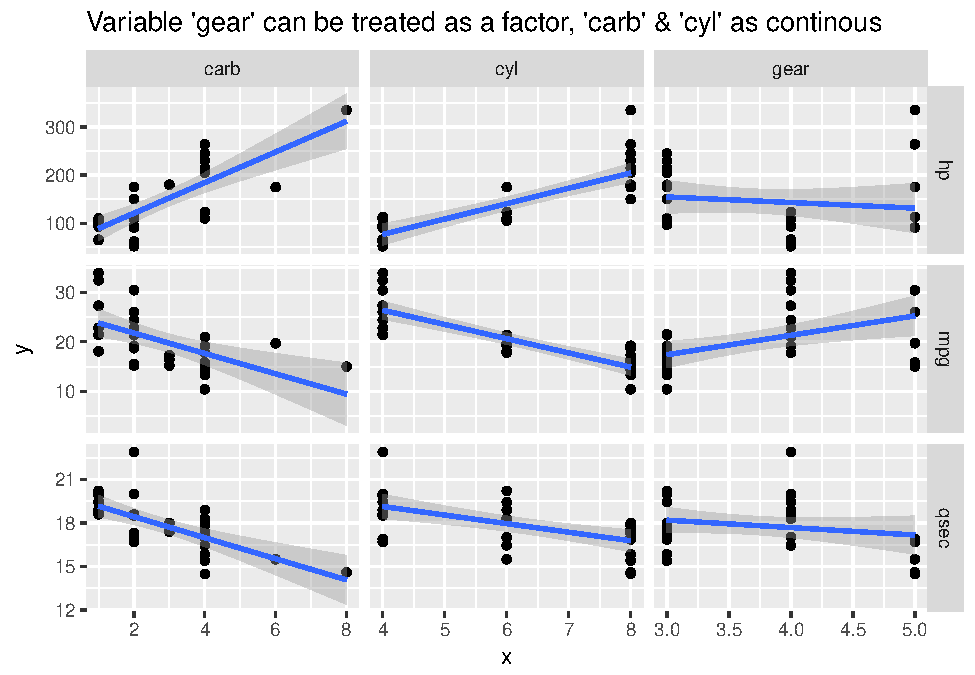
\includegraphics{Regression_Models_Course_Project_files/figure-latex/plot_integer_vars-1.pdf}
\caption{Plot of continuous vs.~factor variables in mtcars data}
\end{figure}

\subsection{Pairs plot for mtcars
dataset}\label{pairs-plot-for-mtcars-dataset}

The pairs plot shows many strong correlations.

\begin{Shaded}
\begin{Highlighting}[]
\NormalTok{if (!}\StringTok{"GGally"} \NormalTok\StringTok{ }\KeywordTok{rownames}\NormalTok{(}\KeywordTok{installed.packages}\NormalTok{())) \{}\KeywordTok{install.packages}\NormalTok{(}\StringTok{"GGally"}\NormalTok{)\}}
\KeywordTok{library}\NormalTok{(GGally)}
\NormalTok{g_pairs <-}\StringTok{ }\KeywordTok{ggpairs}\NormalTok{(mtcars, }\DataTypeTok{mapping=}\KeywordTok{aes}\NormalTok{(}\DataTypeTok{color=}\NormalTok{am, }\DataTypeTok{alpha =} \FloatTok{0.7}\NormalTok{),}
           \DataTypeTok{lower =} \KeywordTok{list}\NormalTok{(}\DataTypeTok{continuous =} \KeywordTok{wrap}\NormalTok{(ggally_smooth, }\DataTypeTok{size =} \DecValTok{1}\NormalTok{)),}
           \DataTypeTok{diag =} \KeywordTok{list}\NormalTok{(}\DataTypeTok{continuous =} \StringTok{"barDiag"}\NormalTok{), }\DataTypeTok{upper =} \KeywordTok{list}\NormalTok{(}\DataTypeTok{continuous =} 
           \KeywordTok{wrap}\NormalTok{(ggally_cor,}\DataTypeTok{size=}\DecValTok{2}\NormalTok{, }\DataTypeTok{mapping=}\KeywordTok{aes}\NormalTok{(}\DataTypeTok{color=}\NormalTok{am,}\DataTypeTok{alpha=}\DecValTok{1}\NormalTok{))), }\DataTypeTok{axisLabels =} \StringTok{'none'}\NormalTok{)}
\KeywordTok{print}\NormalTok{(g_pairs)}
\end{Highlighting}
\end{Shaded}

\begin{figure}[htbp]
\centering
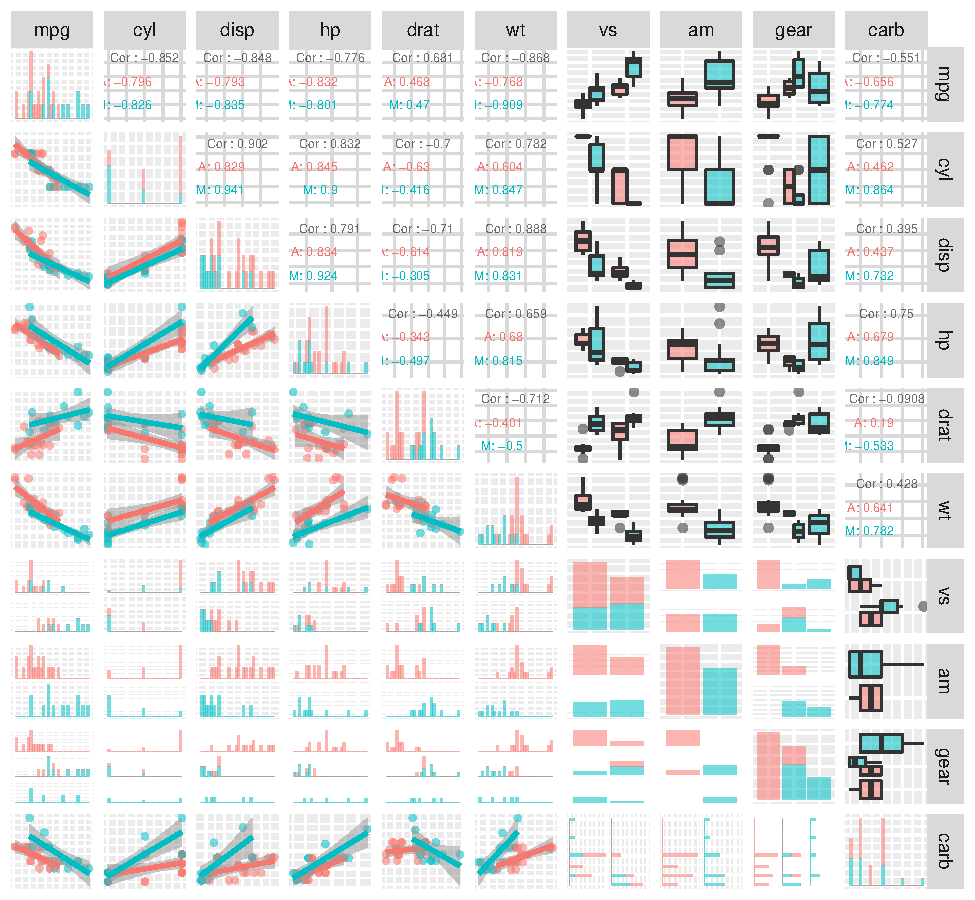
\includegraphics{Regression_Models_Course_Project_files/figure-latex/pairs_plot-1.pdf}
\caption{Pairs Plot of Motor Trend Cars Dataset}
\end{figure}

\subsection{Violin Plot for Manual vs.~Automatic
Transmissions}\label{violin-plot-for-manual-vs.automatic-transmissions}

The violin plot depicts association between transmission type and
\texttt{mpg}.

\begin{Shaded}
\begin{Highlighting}[]
\NormalTok{g_violin <-}\StringTok{ }\KeywordTok{ggplot}\NormalTok{(mtcars, }\KeywordTok{aes}\NormalTok{(}\DataTypeTok{x =} \NormalTok{am, }\DataTypeTok{y =} \NormalTok{mpg)) +}\StringTok{  }
\StringTok{            }\KeywordTok{geom_violin}\NormalTok{() +}
\StringTok{            }\CommentTok{# geom_dotplot(binaxis='y', stackdir='center', dotsize=1) +}
\StringTok{            }\KeywordTok{stat_summary}\NormalTok{(}\DataTypeTok{fun.y=}\NormalTok{mean, }\DataTypeTok{geom=}\StringTok{"point"}\NormalTok{, }\DataTypeTok{shape=}\DecValTok{23}\NormalTok{, }\DataTypeTok{size=}\DecValTok{4}\NormalTok{, }\KeywordTok{aes}\NormalTok{(}\DataTypeTok{fill =} \NormalTok{am)) +}
\StringTok{            }\KeywordTok{scale_fill_discrete}\NormalTok{(}\DataTypeTok{name=}\StringTok{"Mean MPG"}\NormalTok{)+}
\StringTok{            }\KeywordTok{labs}\NormalTok{(}\DataTypeTok{title =} \StringTok{"Average MPG for manual transmissions is significantly higher"}\NormalTok{)}
\KeywordTok{print}\NormalTok{(g_violin)}
\end{Highlighting}
\end{Shaded}

\begin{figure}[htbp]
\centering
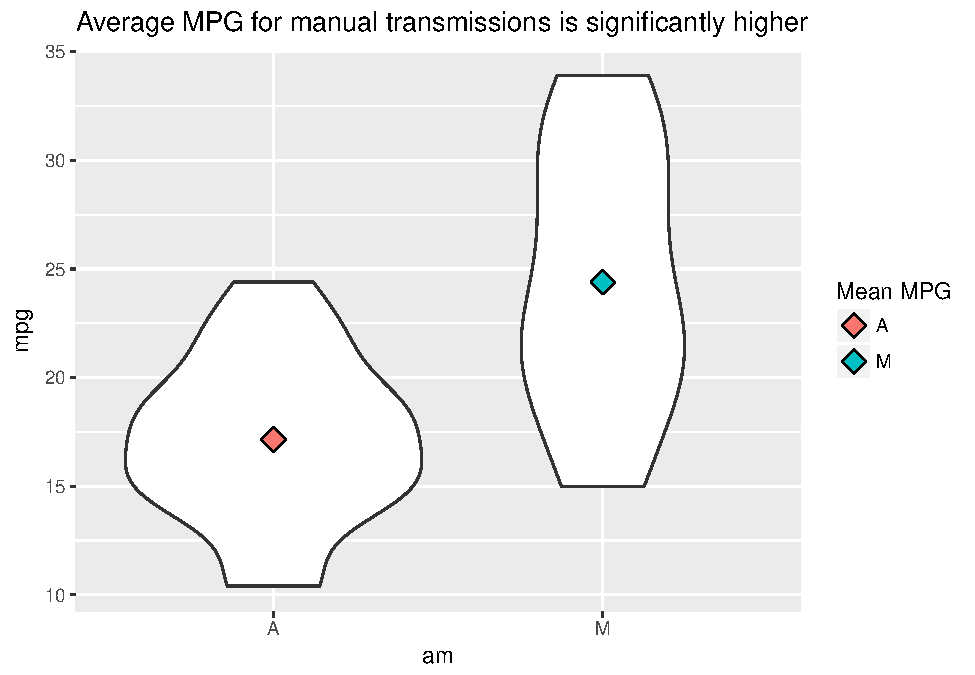
\includegraphics{Regression_Models_Course_Project_files/figure-latex/violin_plot-1.pdf}
\caption{Violin plot of MPG vs.~Transmission type}
\end{figure}

\subsection{Pairs Plot for Variables of Best Constrained and
Unconstrained
Models}\label{pairs-plot-for-variables-of-best-constrained-and-unconstrained-models}

\begin{Shaded}
\begin{Highlighting}[]
\NormalTok{g_model_pairs <-}\StringTok{ }\KeywordTok{ggpairs}\NormalTok{(mtcars[,}\KeywordTok{c}\NormalTok{(}\StringTok{"mpg"}\NormalTok{,}\StringTok{"hp"}\NormalTok{,}\StringTok{"am"}\NormalTok{,}\StringTok{"carb"}\NormalTok{,}\StringTok{"cyl"}\NormalTok{,}\StringTok{"vs"}\NormalTok{,}\StringTok{"wt"}\NormalTok{)], }
                 \DataTypeTok{mapping=}\KeywordTok{aes}\NormalTok{(}\DataTypeTok{color=}\NormalTok{am, }\DataTypeTok{alpha =} \FloatTok{0.7}\NormalTok{),}
                 \DataTypeTok{upper =} \KeywordTok{list}\NormalTok{(}\DataTypeTok{continuous =} \KeywordTok{wrap}\NormalTok{(ggally_smooth, }\DataTypeTok{size =} \DecValTok{1}\NormalTok{)),}
                 \DataTypeTok{diag =} \KeywordTok{list}\NormalTok{(}\DataTypeTok{continuous =} \StringTok{"barDiag"}\NormalTok{), }\DataTypeTok{lower =} \KeywordTok{list}\NormalTok{(}\DataTypeTok{continuous =} 
                 \KeywordTok{wrap}\NormalTok{(ggally_cor, }\DataTypeTok{size=}\DecValTok{3}\NormalTok{, }\DataTypeTok{mapping=}\KeywordTok{aes}\NormalTok{(}\DataTypeTok{color=}\NormalTok{am,}\DataTypeTok{alpha=}\DecValTok{1}\NormalTok{))), }
                 \DataTypeTok{axisLabels =} \StringTok{'none'}\NormalTok{)}
\KeywordTok{print}\NormalTok{(g_model_pairs)}
\end{Highlighting}
\end{Shaded}

\begin{figure}[htbp]
\centering
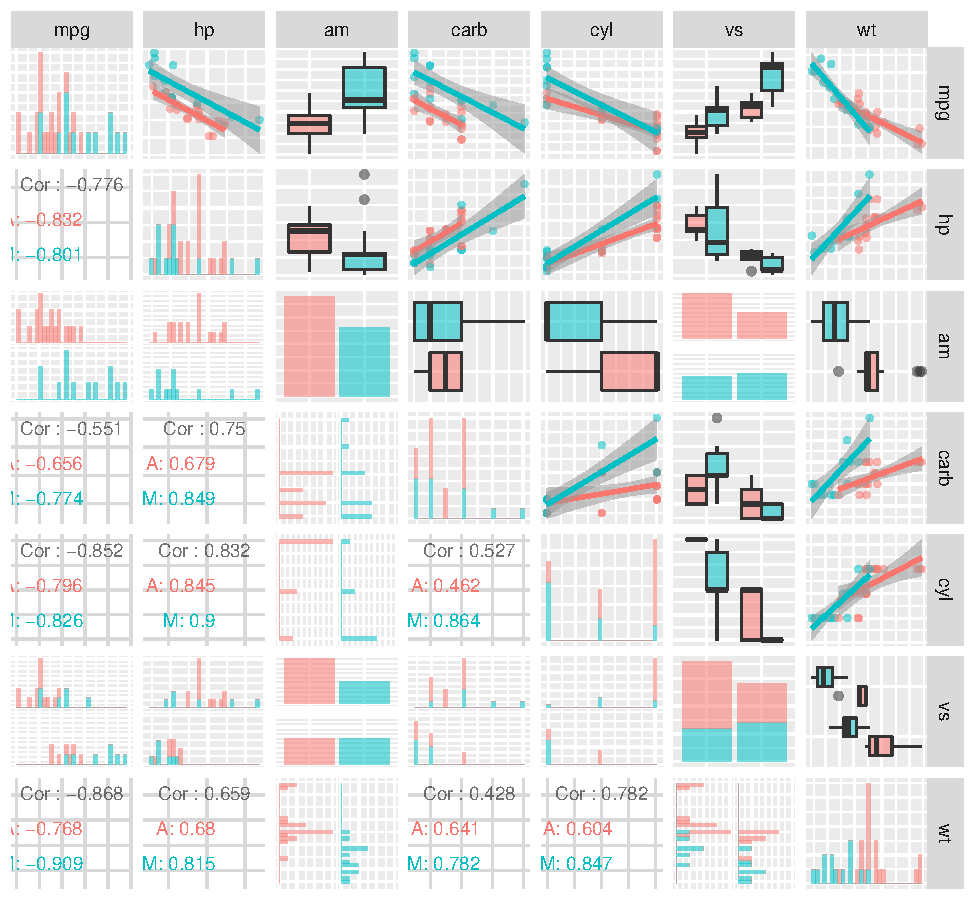
\includegraphics{Regression_Models_Course_Project_files/figure-latex/model_pairs_plot-1.pdf}
\caption{Pairs Plot of Variables of Best Constrained and Unconstrained
Models}
\end{figure}

\subsection{Model Diagnostics}\label{model-diagnostics-1}

\begin{figure}[htbp]
\centering
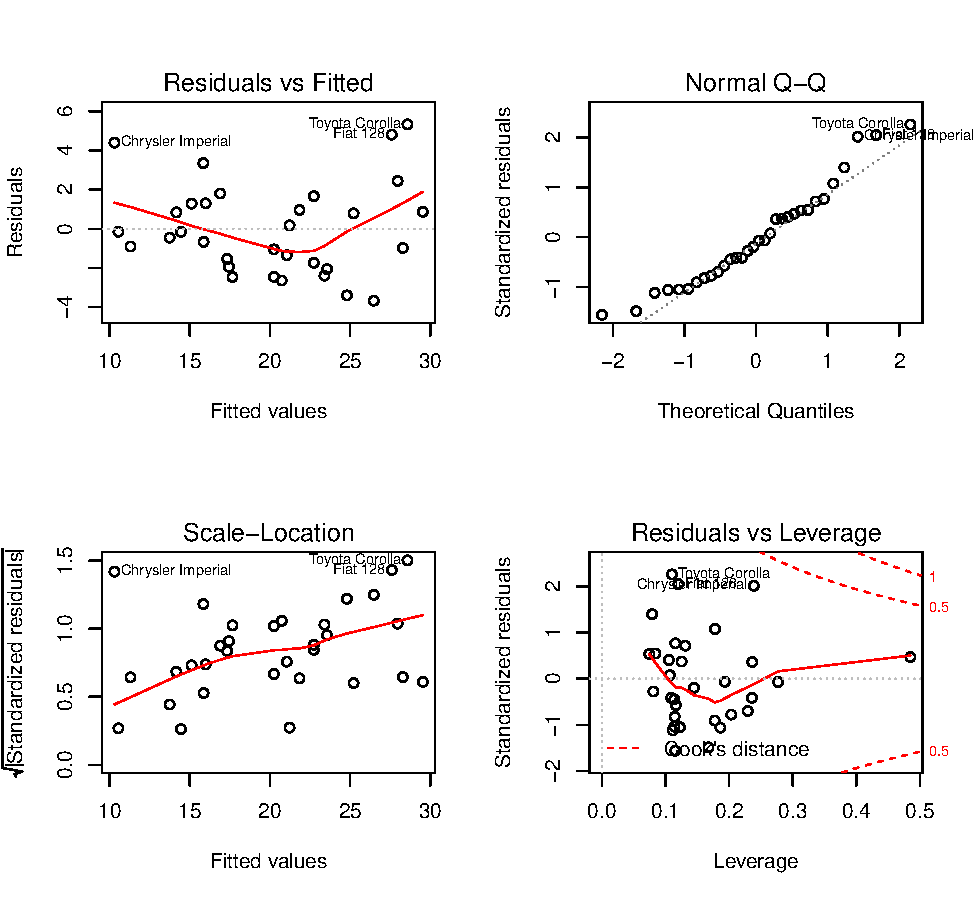
\includegraphics{Regression_Models_Course_Project_files/figure-latex/diagnostics-1.pdf}
\caption{Diagnostic Plots - Best Model that Includes Transmission Type}
\end{figure}

\begin{figure}[htbp]
\centering
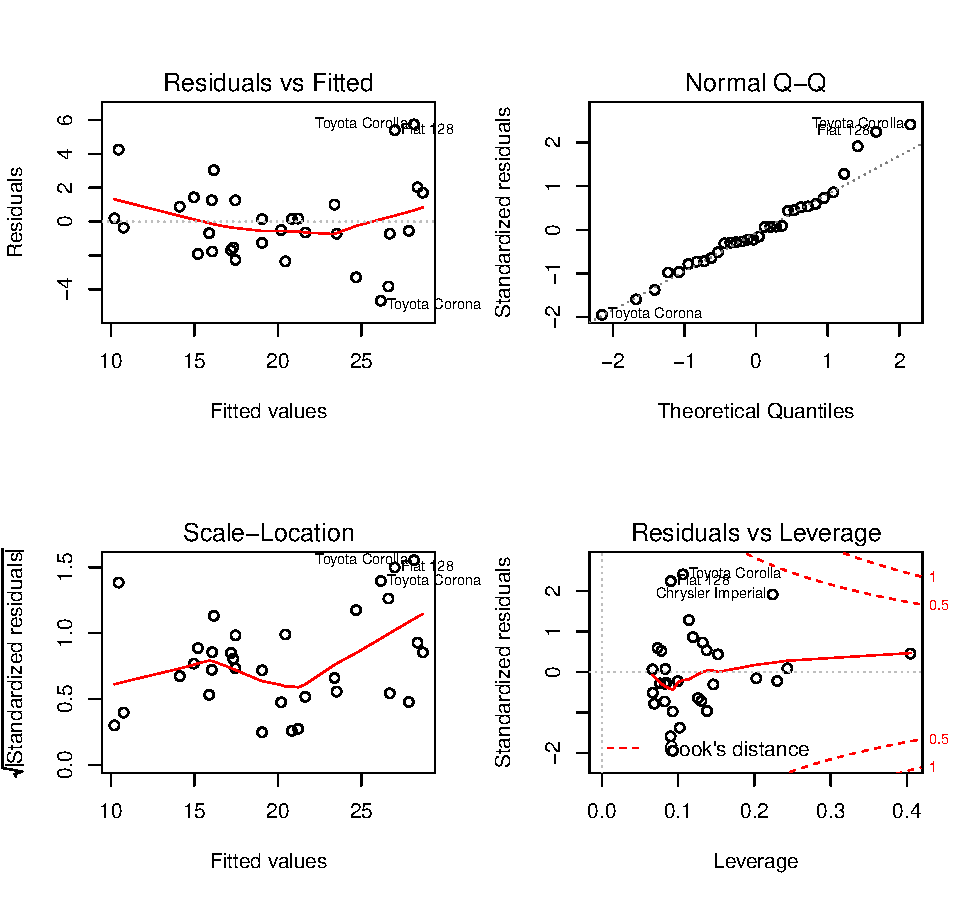
\includegraphics{Regression_Models_Course_Project_files/figure-latex/diagnostics_best_overall_model-1.pdf}
\caption{Diagnostic Plots - Best Overall (Unconstrained) Model}
\end{figure}

\section*{Bibliography}\label{bibliography}
\addcontentsline{toc}{section}{Bibliography}

\hypertarget{refs}{}
\hypertarget{ref-BreimanSubmodelSelection1992}{}
Breiman, Leo, and Philip Spector. 1992. ``Submodel Selection and
Evaluation in Regression: The X-Random Case.'' \emph{International
Statistical Review / Revue Internationale de Statistique} 60 (3).
{[}Wiley, International Statistical Institute (ISI){]}: 291--319.
\url{http://www.jstor.org/stable/1403680}.

\hypertarget{ref-RaoDangersCV2008}{}
Rao, R. Bharat, Glenn Fung, and Romer Rosales. 2008. ``On the Dangers of
Cross-Validation: An Experimental Evaluation.'' In \emph{Proceedings of
the 2008 Siam International Conference on Data Mining}, 588--96.
doi:\href{https://doi.org/10.1137/1.9781611972788.54}{10.1137/1.9781611972788.54}.


\end{document}
